Como se nombró en el objetivo, se busca realizar el control de caudal o presión de un sistema hidráulico. Para esto fue necesario realizar la implementación de un banco de pruebas que cuente de tres partes (Figura \ref{fig:bancofull}).
\begin{itemize}
	\item Soporte para el motor y variador de velocidad,  diseñado y construido por el profesor Gerardo Arthz. A estos elementos se realizó las correspondientes conexiones, y se agregó elementos adicionales: 3 señales luminosas, llave selectora de dos puntos para seleccionar el modo de comunicación, llave selectora de tres puntos (encendido y sentido del motor) y un pulsador de parada de emergencia (Figura \ref{fig:banco}(a)).
	Tanto el motor y los elementos adicionales fueron cableados (Figura \ref{fig:banco}(b)) hacia las borneras del variador de velocidad y se tuvo en cuenta para esto las características y funciones del bornero de control proporcionado por el manual del variador de velocidad\cite{InstaManual}. 
	
	\item Soporte para una bomba en desuso, de características no conocidas con su bobinado quemado.
	\item Circuito hidráulico, que incluye un tanque, válvulas y sensores de caudal y presión.
\end{itemize}




\begin{figure}[htb]
	\centering
	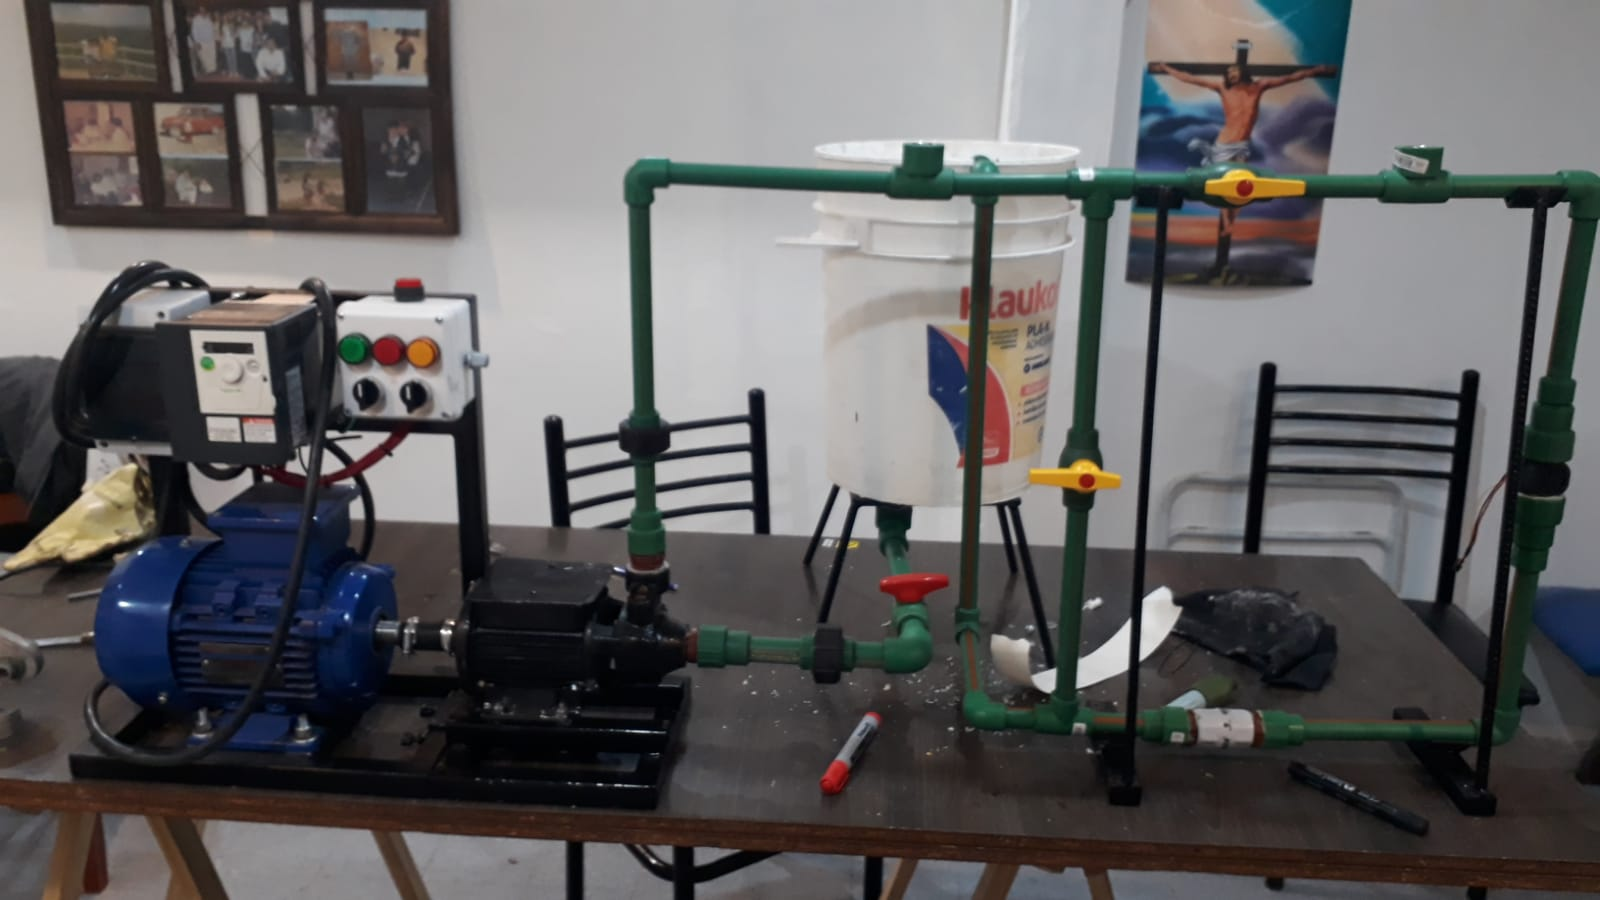
\includegraphics[scale=0.2]{bancofull.png}
	\captionof{figure}{Banco de pruebas completo}
	\label{fig:bancofull}
\end{figure}


\begin{figure}[H]
	\centering
	\subfigure[]{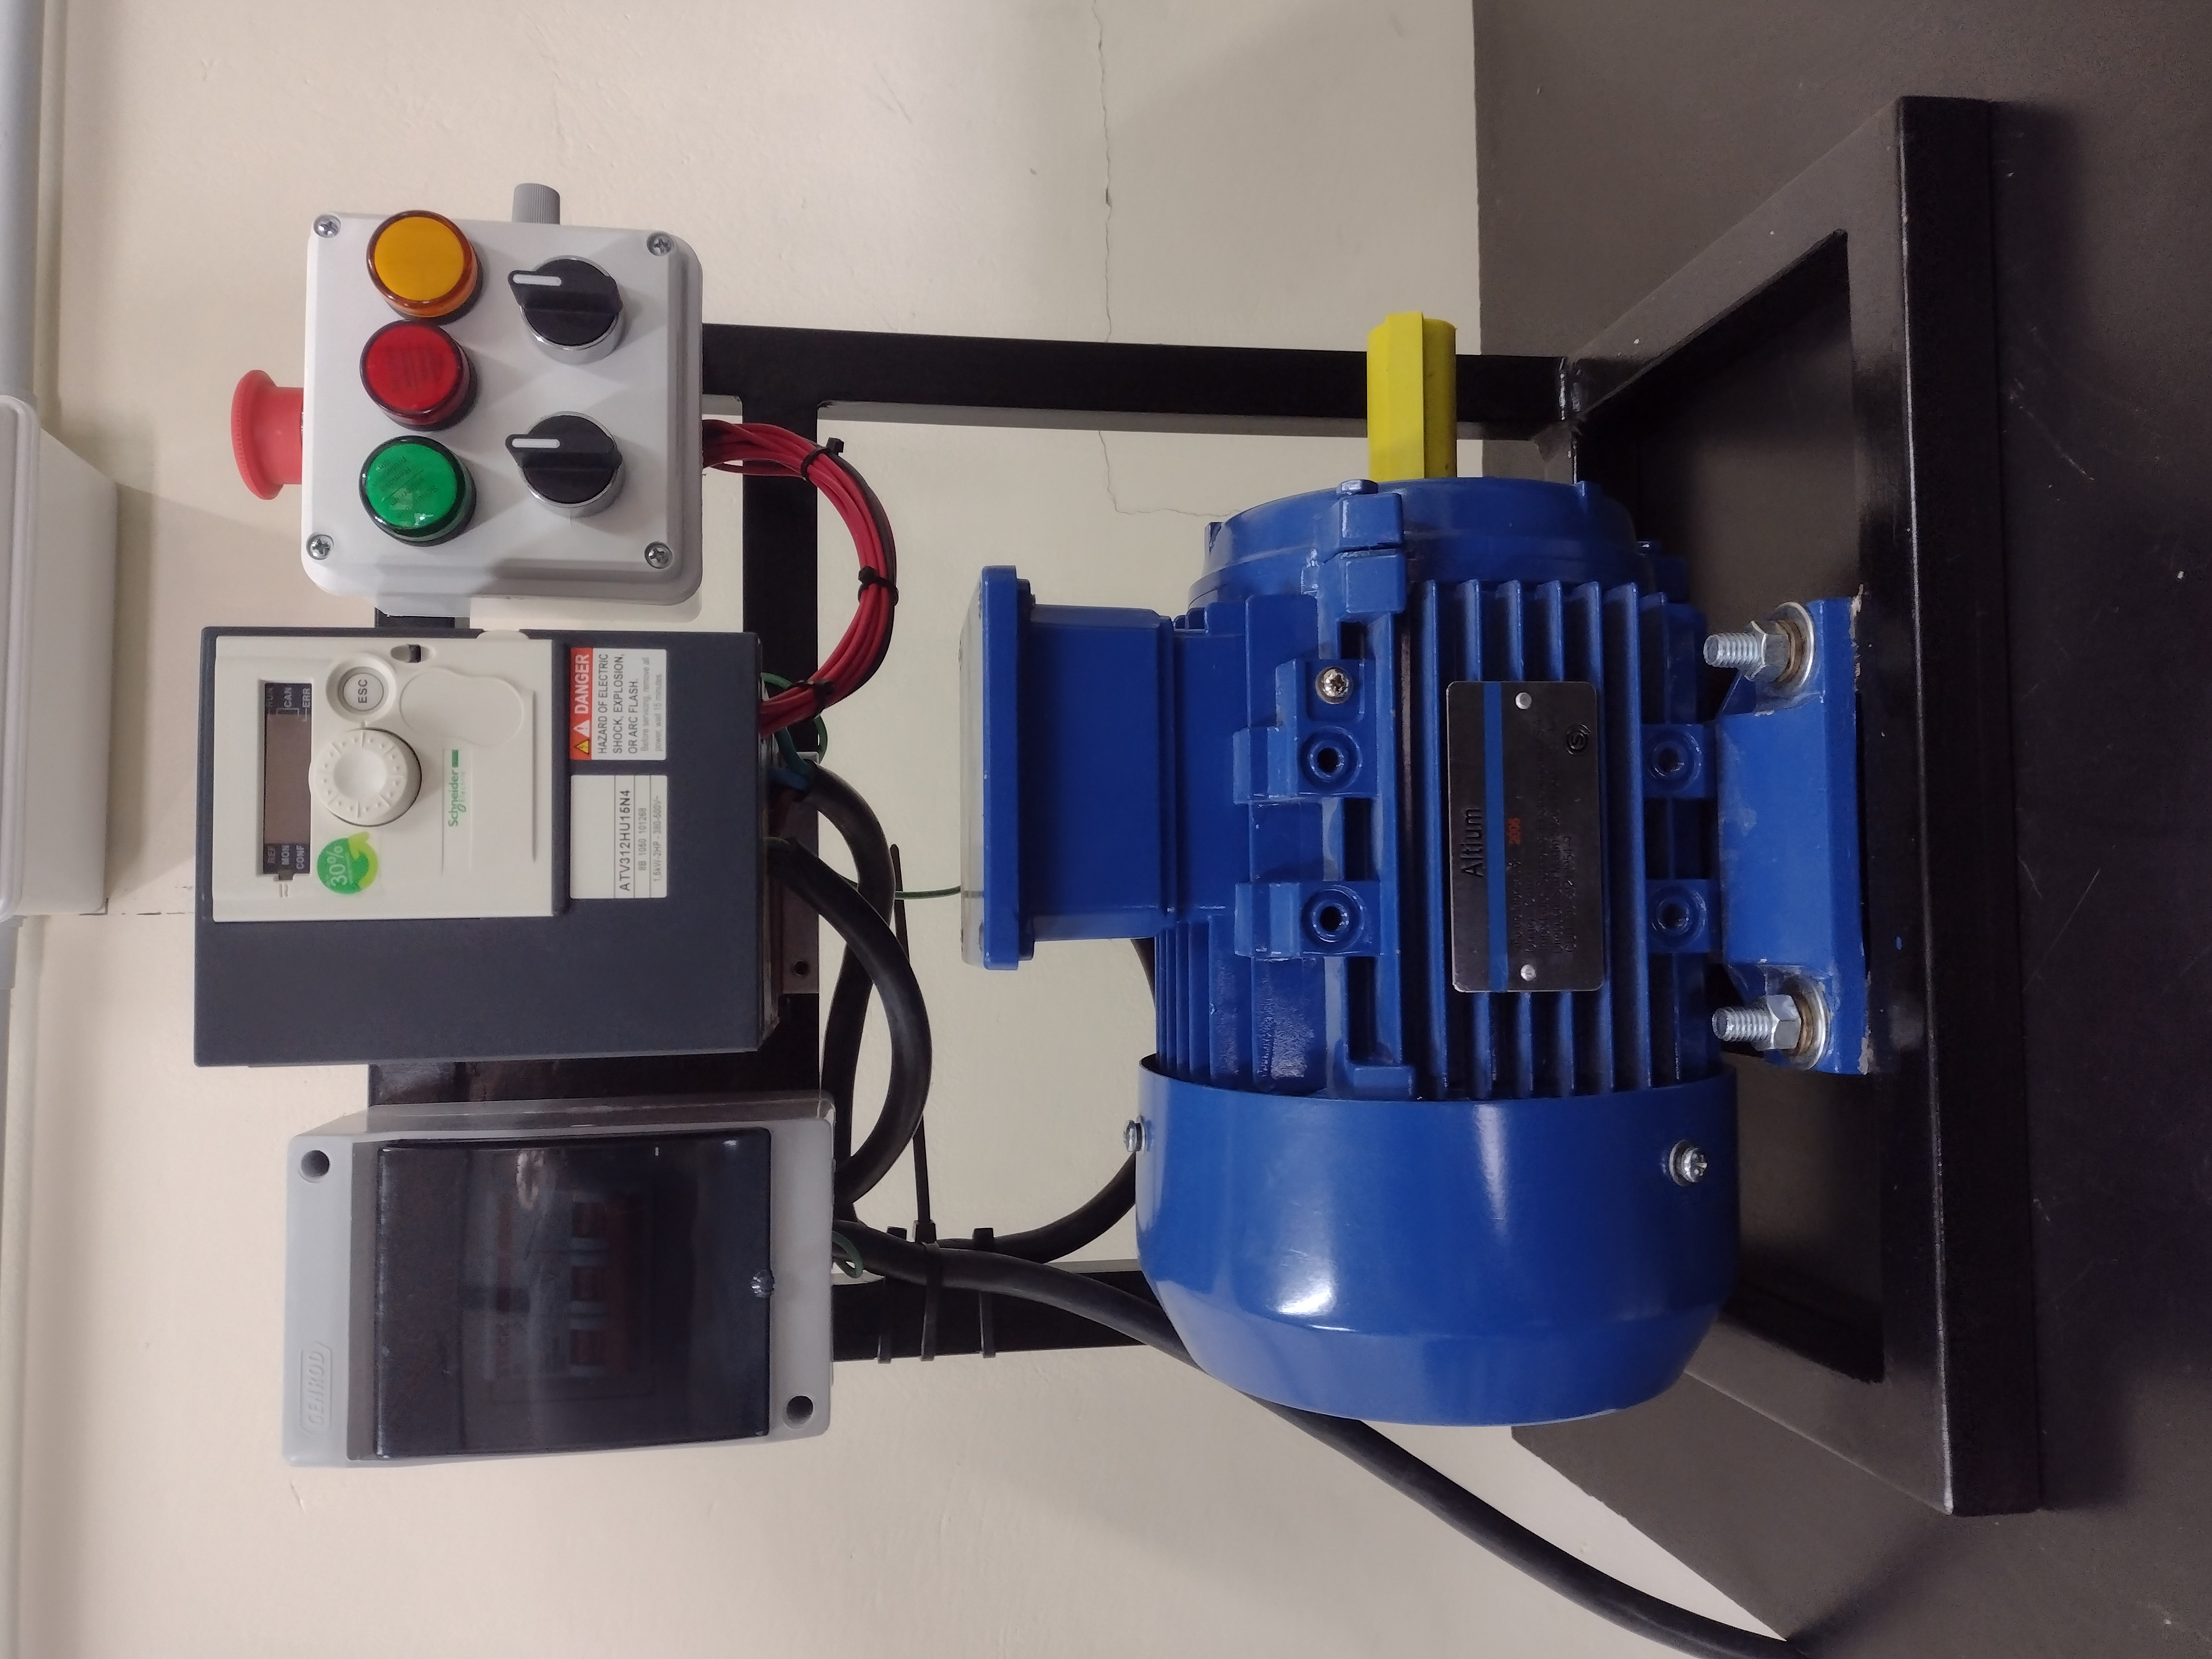
\includegraphics[angle=-90,width=60mm]{banc1 (1)}}
	\subfigure[]{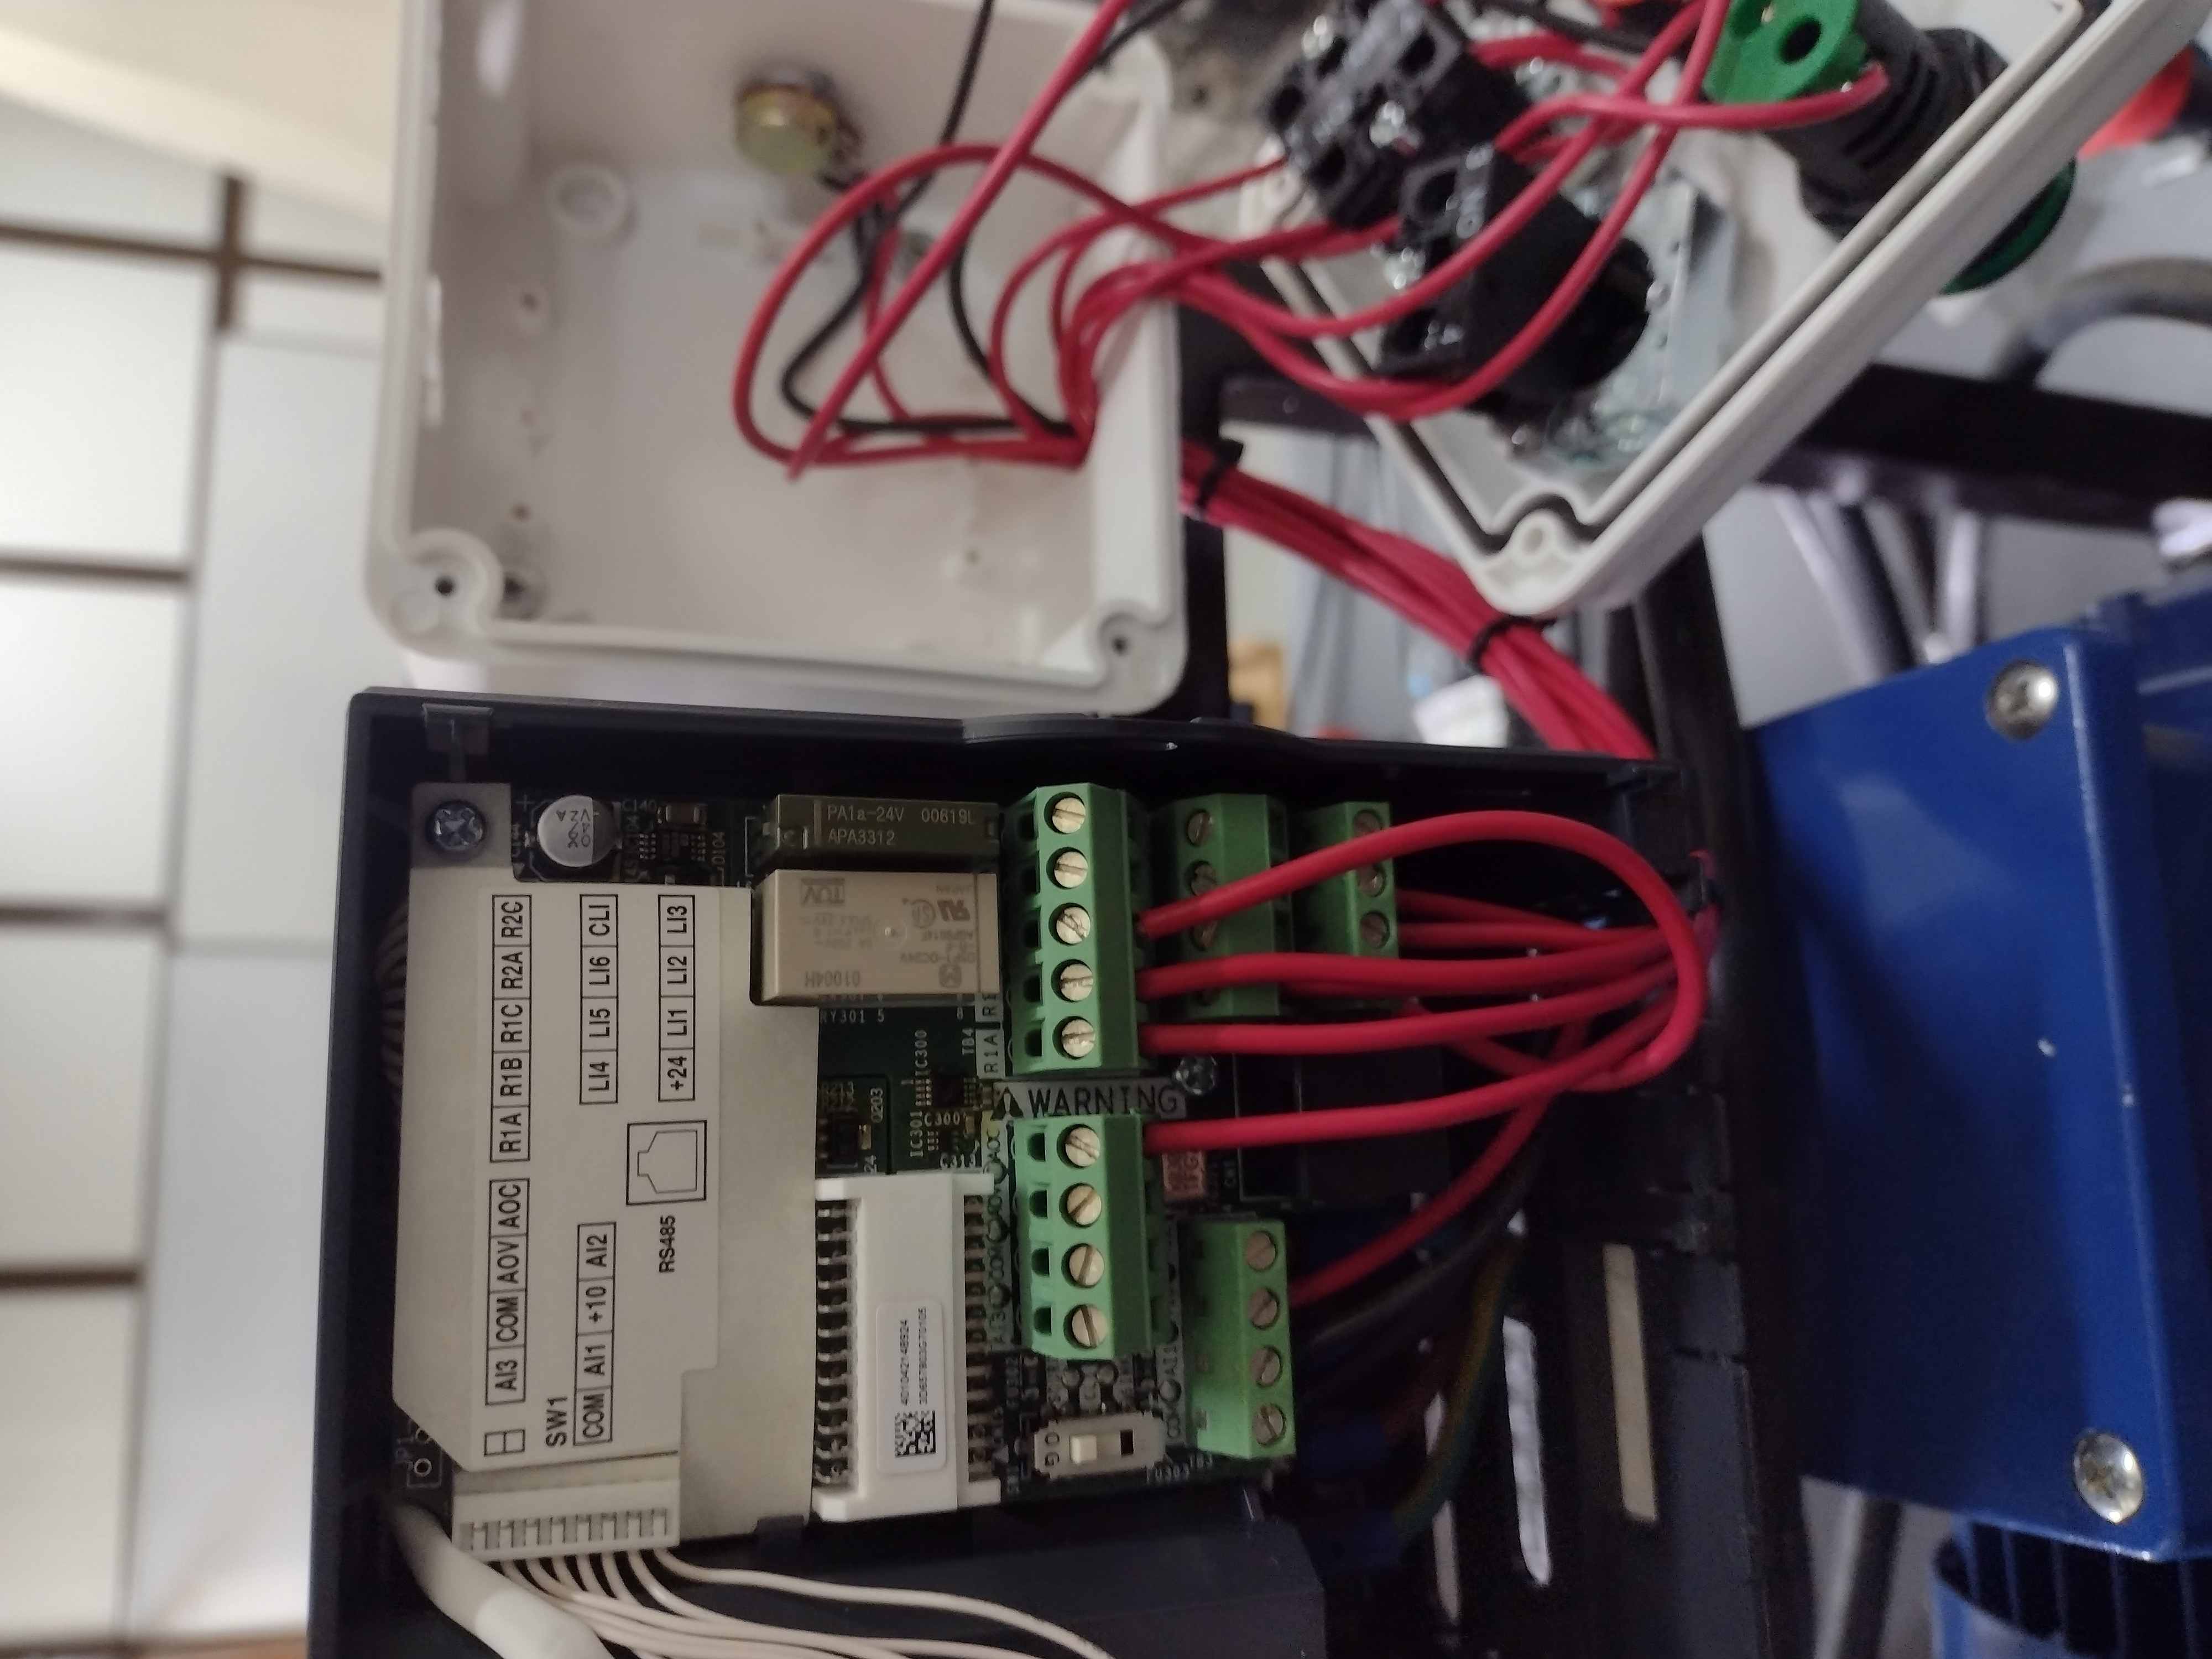
\includegraphics[angle=-90,width=60mm]{images/banc1 (2)}}
	\caption{Banco de Pruebas} \label{fig:banco}
\end{figure}

\subsubsection{Transductor de presión}
Para este proyecto se utilizan dos transductores de presión de montaje en línea modelo EJA530E de la familia  DPharp de Yokogawa (Figura \ref{fig:transd}.a).\\
Las características del EJA530E son:
\begin{itemize}
	\item Precisión: ±0,055\% de precisión
	\item Fiabilidad: ±0,1\% Estabilidad por 10 años
	\item Tiempo de respuesta: 90mseg.
	\item Lazo de corriente de 4-20mA
	\item Se puede configurar en la unidad necesaria, en este caso mBar.
\end{itemize}


\subsubsection{Sensor de caudal}
Se utilizó un sensor de caudal (Figura \ref{fig:transd}.b) genérico con las siguientes características:
\begin{itemize}
	\item Rango de caudal: 2- 60L/min
	\item Máxima presión de agua: 1,75MPa
	\item Conversión de caudal: aprox 477pulsos/L $\pm$ 10\%
\end{itemize}


\begin{figure}[htbp]
	\centering
	\subfigure[Transductor de presión]{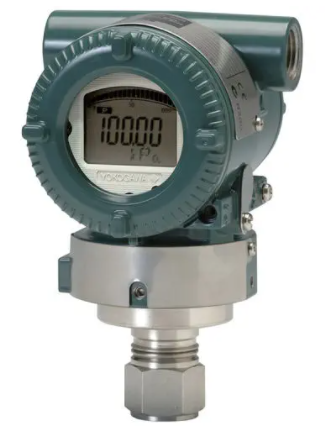
\includegraphics[height=40mm]{tran_pre.png}}
	\subfigure[Sensor de caudal]{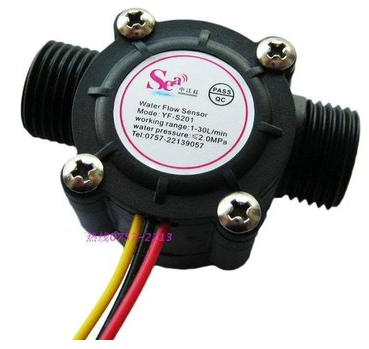
\includegraphics[height=40mm]{sens_pre.png}}
	\caption{Transductores} \label{fig:transd}
\end{figure}





\subsection{Diagrama}
Colocar el diagrama \fcolorbox{red}{yellow}{tipo imagen} pero ver si se agrega el variador y el plc FIGURA\ref{fig:diag}

\begin{figure}[htb]
	\centering
	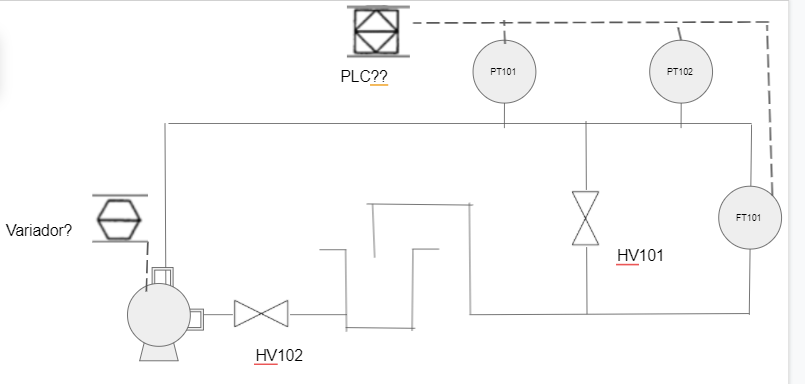
\includegraphics[scale=0.8]{diag.png}
	\captionof{figure}{Diagrama i\&pd}
	\label{fig:diag}
\end{figure}

\subsection{Presupuesto}
\fcolorbox{red}{yellow}{falta lo de la bomba}
\url{https://docs.google.com/spreadsheets/d/1mFoNvgJXUdL2bNnspaBJ_wS5fFA1y1c8fTO9Rfod7H0/edit#gid=0}

\newpage